\documentclass{article}

\usepackage[T1]{fontenc}
\usepackage{lmodern}
\usepackage{graphicx}
\usepackage[margin=1.25in]{geometry}
\graphicspath{ {C:/Users/brent/Downloads/} }
\usepackage[utf8]{inputenc} % allow utf-8 input
\usepackage[T1]{fontenc}    % use 8-bit T1 fonts
\usepackage{hyperref}       % hyperlinks
\usepackage{url}            % simple URL typesetting
\usepackage{booktabs}       % professional-quality tables
\usepackage{amsfonts}       % blackboard math symbols
\usepackage{nicefrac}       % compact symbols for 1/2, etc.
\usepackage{microtype}      % microtypography
\graphicspath{{latex_images}}

\title{Software Tool: Housing Price Visualization}

\author{%
  Brent Christy, Jinyu Liu, Brianna Outen \\
  Northeastern University\\
  Boston, MA 02115 \\
  \texttt{christy.b@northeastern.edu, liu.jinyu@northeastern.edu,} \\
  \texttt{outen.b@northeastern.edu} \\
}

\begin{document}

\maketitle

\section{Problem and Background}
The US housing market is known to be volatile, with prices constantly fluctuating nation-wide and increasing exponentially in regions such as major metropolitan
areas. There are many available housing marketplace platforms and applications that help people search for properties currently on the market but lack
visualizations for important considerations of factors like regional and historical data. The availability of these factors can enable the general population to
make informed decisions for purchasing property based on comparisons of prices in different regions and trends in the real estate market over time. In a market that is subject to change at any point in time, the need for this functionality is becoming increasingly important. 

\subsection{Previous Work}
Zillow is a housing market platform that allows users to view listings in an area by searching an address, neighborhood, city, or zip code. In this tool, the
results are visualized as points on the map of the selected area that display housing prices when moused over. While it is one of the most popular current
available options, Zillow’s functionality is limited. The user can only view current or recent listings and housing prices as individual data points. These points
clutter the visualization and do not provide the users with much information or tools for comparison just by looking at the map since they are all the same size
and color. Important historical pricing data that can be used to identify trends indicating gentrification, investment opportunities, or other considerations is not made available to users with this tool.

\section{Tool Description and Features}
We developed a vizualization software that uses an interactive GUI in order to visualize the housing price data aggregated from Zillow Research datasets. The
pricing data spanned 24 years from 1996 to 2020 and showed the median housing prices for each month in this timeframe for 30,000 zip codes. In order to support the
functionality for visualizing regional data, 7 million data points were aggregated by zip code, county, and state. In the tool, the window
shows the US map generated by shapefiles from the US Census Bureau's geographic census mapping files. These shapefiles contain data points that define the
boundaries of geographic regions so users can view housing prices nation-wide or by narrower parameters from state level down to zipcodes. These prices are shown
on a dynamic color scale where yellow indicates the highest prices and blue indicates the lowest prices as displayed by the color bar to the right of the window.
Two color scale options have been implemented: auto-scale and static mode. If the user selects auto-scale, the software will dynmaically adjust the color bar based
on what is in view in the window. If the user selects the static scale, they have the option to set a scale or keep the scale that is currently in view. 


\section{Software Architecture}
The visualization software is composed of two components, both written in Python. The first 
part is a data pre-processor that parses raw CSV tabular data and converts it into
a normalized, indexed, relational database. The second part of the software is a graphical user interface (GUI) that 
displays the interactive choropleth map to the user. It draws information 
from the database generated by the data pre-processor. This two step process provides an
efficient visualization pipeline and provides a good interactive experience for viewing the housing data.

\subsection{Data Pre-Processor}
\begin{center}
  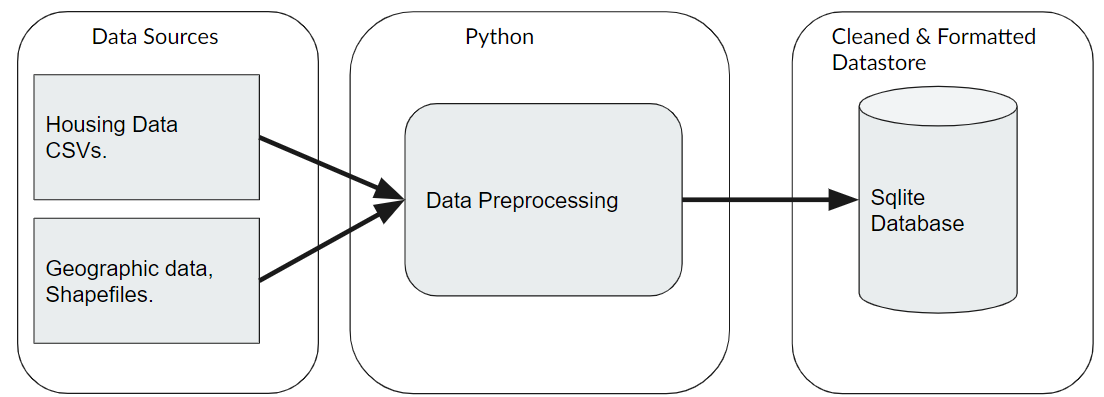
\includegraphics[scale=0.5]{sysarch_pre.png} 
\end{center}  
The data pre-processor is designed to process the tabular housing data into a form more efficient
for the GUI to access. It first downloads the geographic data and housing data from their respective online
sources, the US Census Bureau and Zillow. It then parses the housing data and converts it into a normalized
relational database, splitting the data into multiple tables linked together with keys. This normalization
provides a logical organization of our data and speeds up queries into the database. The pre-processor also
pre-calculates a bounding box, which is the range of longitudes and latitudes that a geographic region occupies,
for all zip codes, counties, and states using the given geographic data. This trades storage space for faster filtering by the GUI. With the 
pre-computed bounding boxes, the GUI no longer needs to calculate the bounding box of each region at runtime,
and can instead just perform a simple query to the database to determine which region's bounding box intersects
with the current region being displayed on the screen. While this process does take around fifteen minutes, it only needs to be performed
once and the outputs don't need to be regenerated unless the data the visualization is based on changes.

\subsection{Visualization GUI}
\begin{center}
  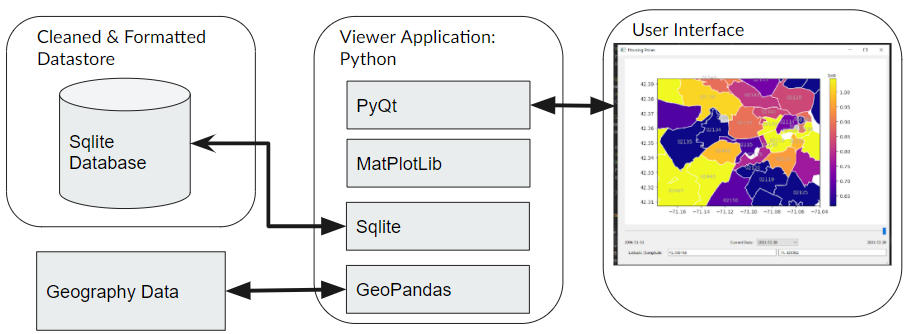
\includegraphics[scale=0.5]{sysarch_gui.png} 
\end{center}  
The GUI is the interactive component of the software. It is a GUI application that paints a choropleth map of
housing values either at the zip code, county, or state level. The map allows dragging when holding down the
center mouse button and zooming using the center mouse button. These actions modify the geographic area that the 
map represents and allows the user to explore housing prices anywhere within the United States. 
To draw the map, the application determines the level of detail to display, either states, counties,
or zip codes based on the current zoom level of the map. Then it queries the database to get a short list of regions
that lay inside of screen, in other word it finds the regions whose bounding box overlaps with that of the screen.
The process quickly determines what regions need to be drawn and greatly reduces the amount of data the GUI program
needs to process to draw the map. We are able to fetch all data and organize them ready to be used by MatPlotLib in
about twenty milliseconds. MatplotLib is then used to plot and color the graph.The process is fairly efficient and achieves 
useable interactivity. The performance of our database based filtering is two orders of magnitude better than Geopanda's
geographic filtering function.
PyQt is used to control other inputs to the GUI such as the current month of data being displayed and what the minimum and maximum values of the colorbar should be.

\section{Insights and Observations}
There are a wide variety of use cases for visualizing aggregated housing data on a map. The spacial mapping of housing information can allow for many comparisons to be made, whether it be across time for observing how quickly prices are changing, or across area for comparing how different prices are in different areas. In the following subsections, several situations will be described where the visualization tool can be used to make decisions and analyze data.

\subsection{Deciding on an Area to Live}
An interesting use case for the software tool is using it to identify an area of the country to live in. A good example is a couple moving to the Boston area. The couple doesn't know much about the area but does know that they have a budget of around \$800,000 to spend on their house. The couple can use our software tool to zoom in on the Boston area to begin. They then can set a static colorbar limit from \$500,000 to \$700,000 on the tool and look around the area. A range of \$500,000 to \$700,000 will show the areas of the region whose median home price is in the range. A bright yellow color will tell the couple that the majority of homes in that zip code are going to be out of their price range. A darker blue color will tell the couple that the homes in that area are probably below their price range. 

\begin{center}
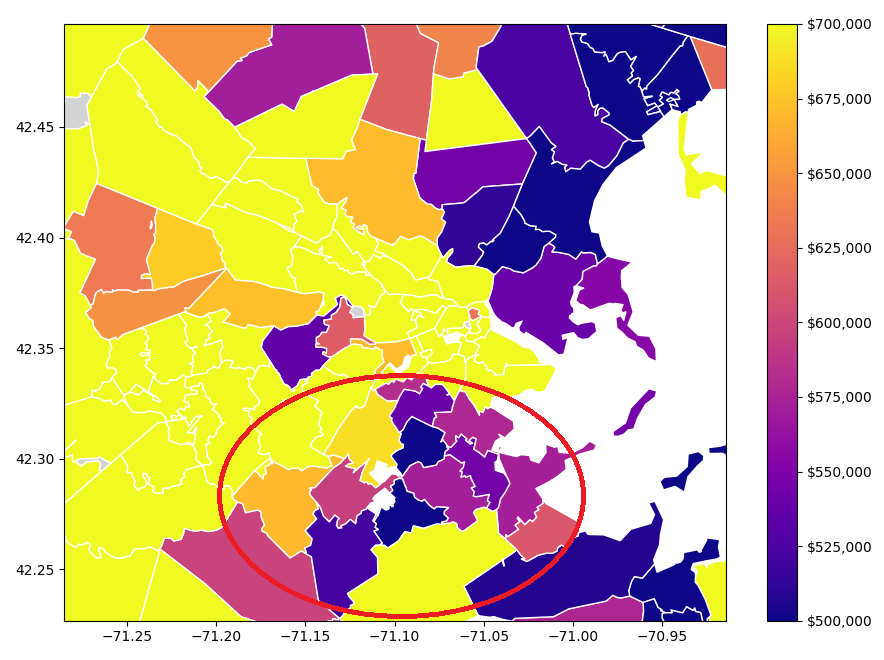
\includegraphics[scale=0.5]{five_hundred_to_seven_hundred.png} 
\end{center}

As can be seen in the color bar in the example above, the range is from \$500,000 to \$700,000. The area that is circled in red south of the city of Boston is a likely area that the couple would identify as a possible place to live. There are many shades between the minimum and maximum in this area and it appears to be a reasonable commute to the city from here. Having identified a reasonable region to live in, the couple may be able to go to a real estate agent with their ideal region picked out, making the process much quicker.

\subsection{Identifying Gentrification}
Another case that the tool could be used for is identifying areas that are becoming gentrified. The feature of the tool that will be used here is adjusting the time being shown. Since the tool has data going all the way back to the year 1996, it is easy to compare how different housing prices are across time periods. This is especially useful for identifying regions of metro areas that are being gentrified. The dynamic color bar is useful for this application.


\begin{center}
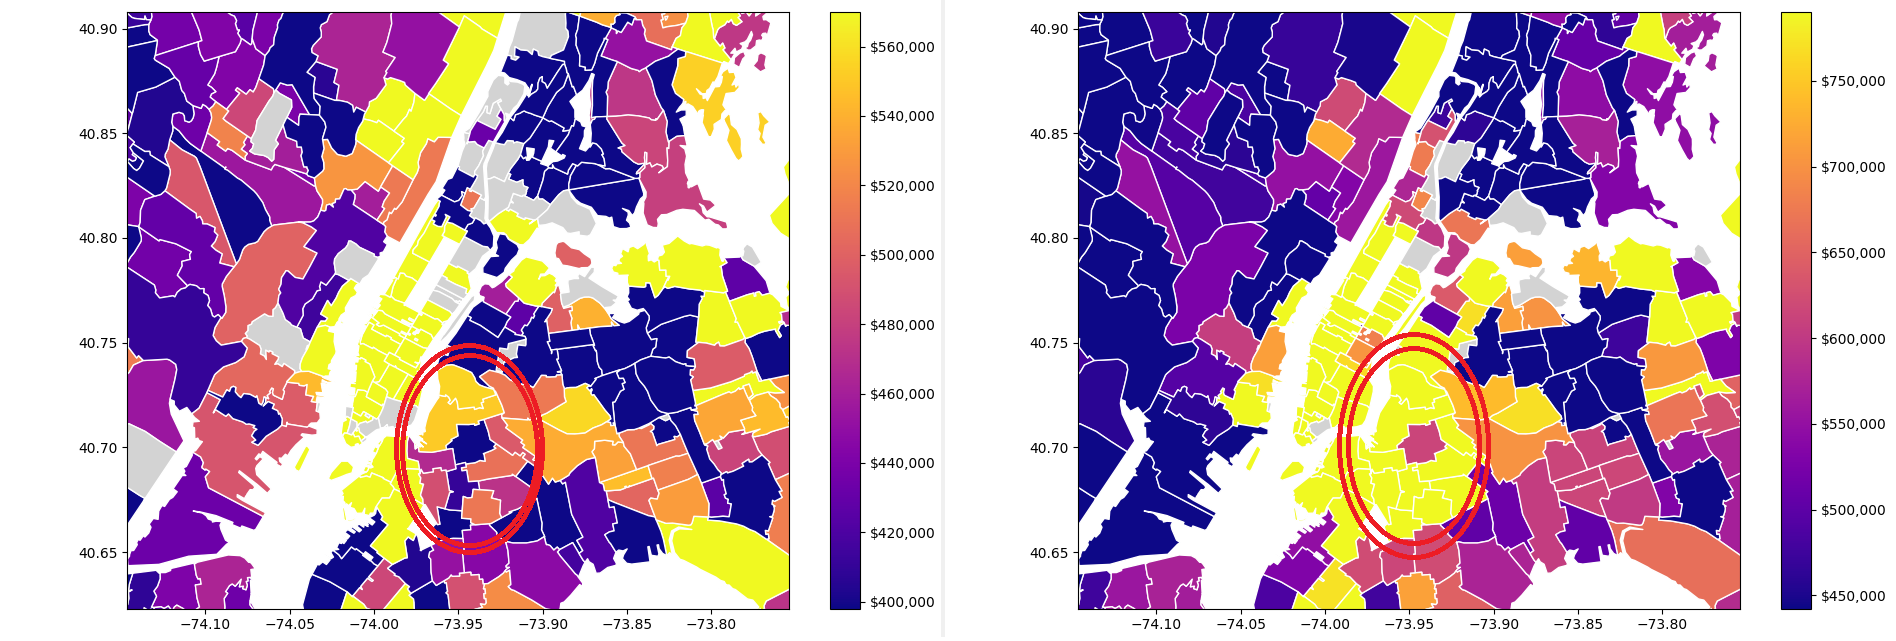
\includegraphics[scale=0.3]{2006_2021_nyc.png} 
\end{center}


The area in red circled above defines an area of Brooklyn including Greenpoint, Williamsburg, and Bushwick. These are areas of Brooklyn well known in the last ten years to have an influx of younger people moving to the area. With younger people moving to the area, the cost of rent and homes will go up accordingly. This can be seen in the images above. Since the color bar is relative in this case, it shows the cost of the homes relative to the areas around it. In the image on the left, 2006, the areas in the circle are darker shades, showing that they are relatively lower than the areas surrounding it. In 2021, the image on the right, you can see that all of the zip codes in the area other than one are now in the highest range of the map, in bright yellow. This tells us that the prices of these homes have moved relatively from being average priced homes in the area to being in the upper percentage of cost in the area. This approach could be taken analyzing areas of any metro area in order to identify and address issues of gentrification.


\section{Future Work}
There are many ways that this work could be expanded in the future. Because of the flexible architecture of the tool, it would be easy to add any kind of numerical metric to the map. Rather than mapping housing prices, something like number of crimes could be visualized as well. The scale would be minimum and maximum crimes committed rather than minimum and maximum of the median home prices. In addition to these, metrics could also be combined to show more advanced statistics such as housing price versus commute time.

There are other features that could have been added to the map to make it more user friendly. Regional markers could be added to help users identify areas of the country better. Regional markers that could be added include cities, towns, and other popular landmarks. In order to make the tool more useful for house hunters, information that could be interesting to a home buyer could be added when clicking on the zip code, such as the schools in the area or community resources.


\end{document}
